%
% Chapter 3
%
\chapter{Proposed Architecture} \label{cap:proposed-architecture}

This chapter presents the proposed architecture for the Remote Lab platform, detailing its main components, their interactions, and the rationale behind the architectural choices.

%
% Section 3.1
%
\section{System Overview} \label{sec31}
The Remote Lab platform is designed as a modular and scalable system, enabling secure and efficient remote access to laboratory equipment. The architecture follows a layered approach, separating concerns between the user interface, application logic, and hardware integration. This separation facilitates maintainability, extensibility, and the integration of new features or laboratory devices.

%
% Section 3.2
%
\section{Main Components} \label{sec32}
The architecture consists of the following main components:
\begin{itemize}
    \item \textbf{Frontend:} A web-based user interface developed with Next.js, providing users with access to laboratory resources, session scheduling, and experiment monitoring.
    \item \textbf{Backend:} Implemented in Kotlin, the backend exposes RESTful APIs for user management, authentication, authorization, and laboratory session control. It also handles business logic and enforces security policies.
    \item \textbf{Hardware Abstraction Layer:} This layer manages communication with laboratory equipment, abstracting hardware-specific details and providing a unified interface for the backend.
    \item \textbf{Database:} Stores user data, session information, access logs, and configuration settings. The database ensures data consistency and supports auditing requirements.
    \item \textbf{Authentication and Authorization:} Ensures secure access to the platform, supporting multiple user roles (e.g., students, professors, administrators) with different permissions.
\end{itemize}

%
% Section 3.3
%
\section{Component Interactions} \label{sec33}
The components interact as follows:
\begin{itemize}
    \item Users interact with the frontend to authenticate, schedule sessions, and access laboratory resources.
    \item The frontend communicates with the backend via secure API calls.
    \item The backend processes requests, applies business logic, and interacts with the database and hardware abstraction layer as needed.
    \item The hardware abstraction layer translates backend commands into device-specific instructions, enabling remote control of laboratory equipment.
\end{itemize}

%
% Section 3.4
%
\section{Architecture Diagram} \label{sec34}
Figure~\ref{fig:architecture} illustrates the high-level architecture of the Remote Lab platform.

% Insert architecture diagram here
\begin{figure}[h]
\begin{center}
    \resizebox{100mm}{!}{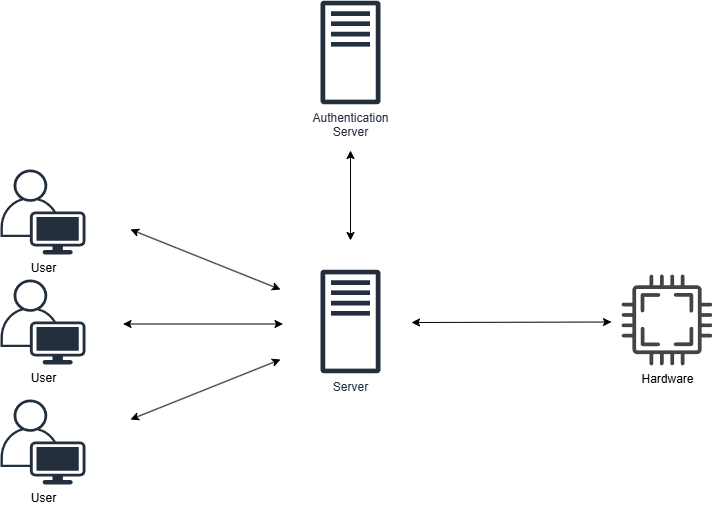
\includegraphics{./../img/SimpleArchitectureRL.drawio.png}}
\end{center}
\caption{High-level architecture of the Remote Lab platform.}\label{fig:architecture}
\end{figure}

%
% Section 3.5
%
\section{Design Rationale} \label{sec35}
The architectural choices were guided by the need for scalability, security, and ease of integration with diverse laboratory equipment. The use of a layered architecture and standardized interfaces ensures that the platform can evolve to meet future requirements and support additional functionalities.